\chapter{Introduction (Heading level 1)}\label{introduction}
    \section{Heading level 2}\label{sec:level2}
        \subsection{Heading level 3}\label{subsec:level3}
        The bullets will be offset by 1cm with the first line being pushed by 0.6cm
        (applied to the text~\cite{appdesigner} after a bullet, exceeding one line). The tab will be
        set at a distance of 1.6 cm with left alignment. Set the space before paragraph
        to 3pt~\ref{fig:example}:
        \begin{itemize}
            \item indent one,
            \item indent two,
            \item indent three,
        \end{itemize}
    \section{Figures}\label{sec:figures}
    The figures will be centered, with a 10pt blank space above and
    under the figure~\cite{Levinson}. Under the center-aligned picture, the description
    of the figure shall be inserted (Arial, 10pt spacing, bold),
    labeled as "Fig.“. ~\ref{fig:example}
    \begin{center}
        \begin{figure}[!ht]
            \centering
            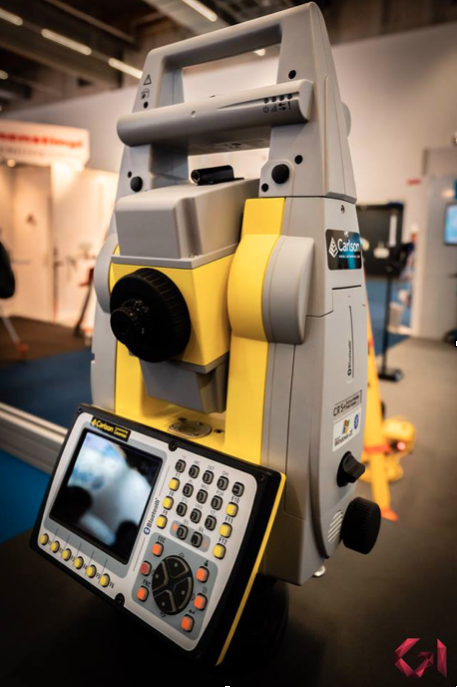
\includegraphics[width=0.2\textwidth]{figures/example}
            \caption{Robotic total station}
            \label{fig:example}
        \end{figure}
    \end{center}
    \section{Tables}\label{sec:tables}
    The tables should also be centered. The table description will be
    placed in front of the table and written in Arial, font size 10pt,
    bold, with 10pt~\cite{Durbin} blank space before and after. The description of
    the table will be labeled "Tab."~\ref{tab:example}.
    \begin{table}[!ht]
        \centering
        \begin{tabular}{|l|c|}
            \hline
            Column 1 & Column 2 \\
            \hline
            Monday & 1 \\
            Tuesday & 2 \\
            Wednesday & 3 \\
            Thursday & 4 \\
            Friday & 5 \\
            \hline
        \end{tabular}
        \caption{Working days}
        \label{tab:example}
    \end{table}
    \section{Example of equation numbering}\label{sec:equation}
    \begin{equation}
        a + b + c = d
    \end{equation}
